\section{Теоремы о предельных значениях}
\begin{theorem}
Пусть $f$ --- непрерывно-дифференцируемая функция и \(f(t) \supset F(p)\), cуществует \(f(+\infty)\); тогда \(f(+\infty) = \lim_{p \rightarrow 0} pF(p)\).
\end{theorem}
\begin{proof}
 \[
 	f'(t) \supset pF(p) - f(+0)
 \]
 \[
 	\int \limits_0^{+\infty}f'(t)e^{-pt} \, dt = pF(p)-f(+0)
 \]
 При \(p \rightarrow 0\) выражение \(\rightarrow f(+\infty)-f(+0)\).\\
 
 \[
 	\cos t \supset \dfrac{p}{p^2+1} \quad \sin t \supset \dfrac{1}{p^2+1} 
 \]
 \[
 	pF(p) = \dfrac{p^2}{p^2+1} \rightarrow 0 (p\rightarrow0)
 \]
  \[
 	pF(p) = \dfrac{p^2}{p^2+1} \rightarrow 1 (p\rightarrow \infty)
 \]
   \[
 	\dfrac{p}{p^2+1} \rightarrow 0 (p\rightarrow \infty)
 \]
 \end{proof}
 \begin{theorem}
 Пусть $f$ --- непрерывно-дифференцируема;  \(f(t) \supset F(p)\) и существует \(f(+0)\). 
 Тогда \(f(+0) = \lim_{p\rightarrow +\infty} pF(p)\).
 \end{theorem}
 \begin{proof}
 \[
 	\int \limits_0^{+\infty} f'(t) e^{-pt}\, dt = pF(p) - f(+0)
 \]
\end{proof}
\clearpage
\section{Приложения преобразования Лапласа к исследованию процессов в электрических цепях}
\[
	i \supset I, \quad e \supset E.
\]
\begin{center}
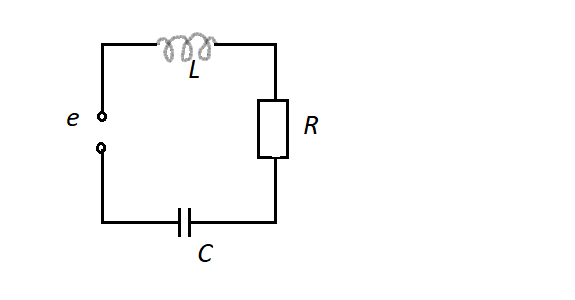
\includegraphics[width=10cm, height=5cm]{ch12/10}
\end{center}
\[
	U_L=L \dfrac{di}{dt}
\]
\[
	U_R = Ri
\]
\[
	U_C = \dfrac{1}{C} \int \limits{0}{t}i(t) \, dt
\]
Пусть \(i(0)=0\).\\
\[
	L\dfrac{di}{dt} + Ri+\dfrac{1}{C} \int \limits{0}{t}i(r) \, dr = e(t)
 \]
 \[
 	pLI + RI + \dfrac{I}{Cp} = E
 \]
 \[
 	(pL+R+\dfrac{1}{Cp})I = E,
 \]
\(Z = pL+R+\dfrac{1}{Cp}\) --- импеданс(операторное сопротивление), \(Y=\dfrac{1}{Z}\) --- адмитанс.\\
\begin{center}
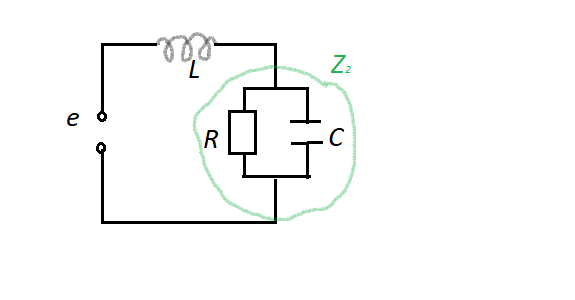
\includegraphics[width=10cm, height=5cm]{ch12/11}
\end{center}
\[
	Z = Z_1 + Z_2
\]
\[
	\dfrac{1}{R} + \dfrac{1}{\frac{1}{Cp}} = \dfrac{1}{Z_2}
\]
\[
	C_p + \dfrac{1}{R} = \dfrac{CR_P + 1}{R}
\]
\[
	Z_2 = \dfrac{R}{CR_p + 1}
\]
\[
	Z= pL = \dfrac{R}{CR_p+1}
\]
При параллельном соединении:
\[
	Z_1...Z_n;
\]
\[
	Y_1 = \dfrac{1}{Z_1}...Y_n = \dfrac{1}{Z_n}
\]
\[
	Y = Y_1 + ... + Y_n
\]
\begin{center}
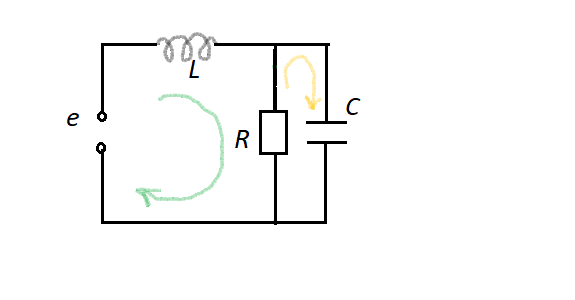
\includegraphics[width=14cm, height=7cm]{ch12/12}
\end{center}

Рассмотрим схему как двухконтурную(закон Кирхгофа):
\[
	\begin{cases}
		pLI_1 + R(I_1-I_2)=E\\
		R(I_2-I_1) + \dfrac{1}{Cp}I_2 = 0
	\end{cases}
\]
\[
	I_2(R + \dfrac{1}{Cp}) - RI_1 = 0
\]
\[
	I_2 = \dfrac{R}{R+\frac{1}{Cp}}I_1
\]
\[
	I_1- I_2 = \left(1 -   \dfrac{R}{R+\frac{1}{Cp}} \right) I_1 = \dfrac{\frac{1}{Cp}}{R + \frac{1}{Cp}}I_1 = \dfrac{1}{CR_p+1}I_1
\]
\[
	I_1(pL + \dfrac{R}{CR_p+1})=E
\]
\[
	I_1Z=E
\]
\begin{enumerate}
\item Постоянный ток
\[
	l=l_0 \quad E=\dfrac{l_0}{p}
\]
\item Переменный ток
\[
	l = l_0 \sin \omega t \quad E = \dfrac{l_0 \omega}{p^2 + \omega^2}
\]
\end{enumerate}
\[
	(L_p + R + \dfrac{1}{Cp}) = \dfrac{l_0}{p}
\]
\[
	I = \dfrac{l_0}{p}\left( \dfrac{1}{L_p + R + Cp} \right) = \dfrac{l_0 C p}{p(CLp^2 + RCp + 1)} = \dfrac{l_0}{(Lp^2+Rp+\frac{1}{C}}=
\]
\[
	= \dfrac{l_0}{(L(p+\frac{R}{2L})^2-\frac{R^2}{4L} + \frac{1}{C}}.
\]
\[	
	D = C^2R^2 - 4CL
\]
Пусть \( C^2R^2 - 4CL < 0 \Rightarrow \)  комплексные корни.\\
\[
\dfrac{l_0}{(L(p+\frac{R}{2L})^2-\frac{R^2}{4L} + \frac{1}{C}} = \dfrac{l_0C}{CLp^2 + \frac{2\sqrt{CL}}{2\sqrt{CL}}+\dfrac{(CR)^2}{4CL}-\dfrac{CR^2}{4CL} +1} =
\]
\[
	= \dfrac{Cl_0}{(\sqrt{CL}p + \frac{CR}{4\sqrt{CL}})^2 - \dfrac{CR^2}{4CL} +1} = \dfrac{l_0 C/CL}{(p+\frac{R}{2L})^2 +\frac{1-\frac{CR^2}{4L}}{CL}}
\]
\[
	\dfrac{l_0}{L(p+\frac{R}{2L})^2 - \frac{R^2}{4L} + \frac{1}{C}} = \dfrac{l_0/L}{(p+\frac{R}{2L})^2  + (\dfrac{1}{CL}-\frac{R^2}{4L^2})} < e^{-\frac{R}{2L}t}\dfrac{l_0}{L} \sin  \dfrac{\sqrt{(\frac{1}{CL}-\frac{R^2}{4L^2})t}}{\sqrt{\frac{1}{CL}-\frac{R^2}{4L^2}}}
\]